 \documentclass[acmtog,anonymous,review]{acmart}
\acmSubmissionID{401}
\usepackage{graphicx}


\date{}
\title{Supplemental Material for "Bijective and Coarse High-order Tetrahedral Meshes"}
\begin{document}
\maketitle

\section*{Additional Comparison with Curved Optimal Delaunay Triangulation}

For completeness, we include all the results generated by the Curved ODT authors for our comparison. 

The authors of Curved ODT processed a total of 4 models for our comparison: two organic (Figure~\ref{bichon:fig:smooth}) (1) gargoyle, (2) dancer, and two mechanical (Figure~\ref{bichon:fig:features}) (3) octa, (4) Team2. The tetrahedra in orange in the figures have negative Jacobian determinant.

The models were processed by the authors using their reference implementation, using a target of 10k vertices and a sizing field. The algorithm worked on models (1) and (2) generating 38159 and 36044 tetrahedra (Figure 21 of our paper). In comparison our algorithm can mesh these two models using 2037 and 2179 tetrahedra, respectively. For the methods with features ((3) and (4)) CODT could not converge, generating meshes with missing features and inverted tetrahedra. The meshes they generated have 
 36622 and 35878 tetrahedra, respectively.
Our algorithm can mesh (3) and (4) with 1063 and 6322 tetrahedra, respectively.

The authors also run the algorithm with a budget of 1k vertices. The algorithm failed to converge on models (1) and (2) and was not deemed worthy to try it on models (3) and (4) as they are too complex for that element budget. Curved ODT has a mechanism to mitigate the number of inverted tetrahedra called ``sliver peeling'' (remove tetrahedra with 2 boundary faces) controlled by an angle. Unfortunately, for this low budget of vertices, either the default angle or $150^\circ$ did not help.

% Dancer v 555 t 2179
% Gargo (2037, 35) (492,)
% Team (6322, 35) (1431,)
% Octa (1063, 35) (262,)



\begin{figure}
    \centering
       \includegraphics[width=.24\linewidth]{addional_figs/gargo_peel.png}\hfill
    \includegraphics[width=.24\linewidth]{addional_figs/gargo_peel_150.png}
    \hfill
    \includegraphics[width=.24\linewidth]{addional_figs/dancer_peel.png}\hfill
    \includegraphics[width=.24\linewidth]{addional_figs/dancer_peel_150.png}\hfill
    \parbox{.24\linewidth}{\centering Default
    peeling}\hfill
    \parbox{.24\linewidth}{\centering $150^\circ$ peeling}\hfill
    \parbox{.24\linewidth}{\centering Default
    peeling}\hfill
    \parbox{.24\linewidth}{\centering $150^\circ$ peeling}
    \caption{Output of Curved ODT on organic models}
    \label{bichon:fig:smooth}
\end{figure}

\begin{figure}
    \centering
    \includegraphics[width=.45\linewidth]{addional_figs/octa.png}
    \includegraphics[width=.45\linewidth]{addional_figs/mech.png}
    \caption{Example of models with sharp features where the LFS is suboptimal and CODT cannot generate valid curved tetrahedral meshes.}
    \label{bichon:fig:features}
\end{figure}


\begin{figure}
    \centering
    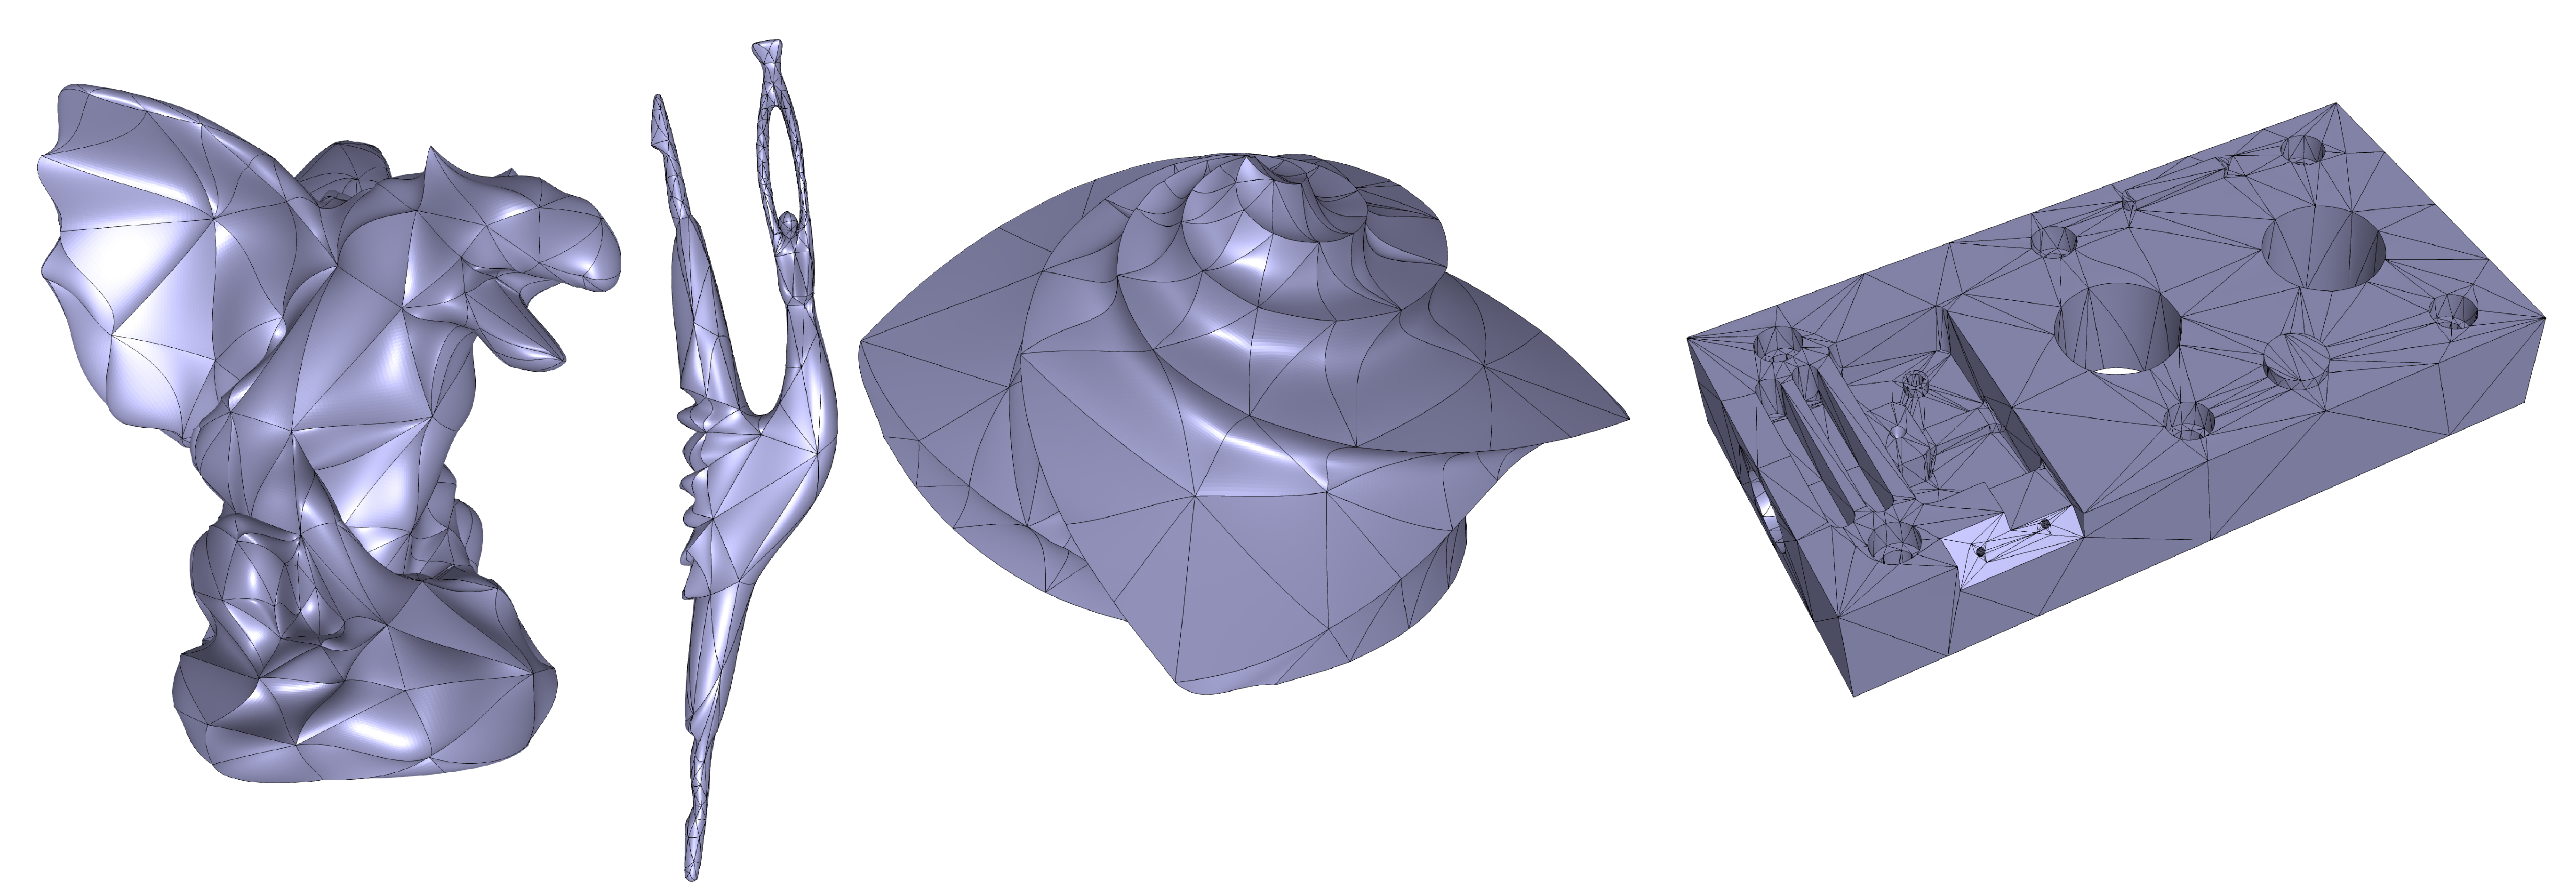
\includegraphics[width=.9\linewidth]{addional_figs/additional_mp.pdf}
    \caption{Our results.}
\end{figure}
\end{document}